
% --- Bắt đầu SECTION: GIỚI THIỆU & BỐI CẢNH ---
\section{I-DẪN NHẬP VÀ TỔNG QUAN}

% --- Slide 3: Vấn đề toàn cầu ---
\begin{frame}{Té ngã: Vấn đề chung toàn cầu}
    \begin{columns}[T]
        \begin{column}{0.48\textwidth}
            \begin{itemize}
                \item Nguyên nhân chính gây chấn thương và tử vong không cố ý.
                \item \textbf{WHO}: $\sim646,000$ ca tử vong/năm; $>80\%$ ở các nước thu nhập trung bình/thấp.
                \item Người cao tuổi: \textbf{30\%} té ngã/năm ở người $>65$ tuổi, tăng lên \textbf{50\%} ở người $>85$ tuổi.
            \end{itemize}
        \end{column}
        \begin{column}{0.48\textwidth}
            \begin{figure}
                \centering
                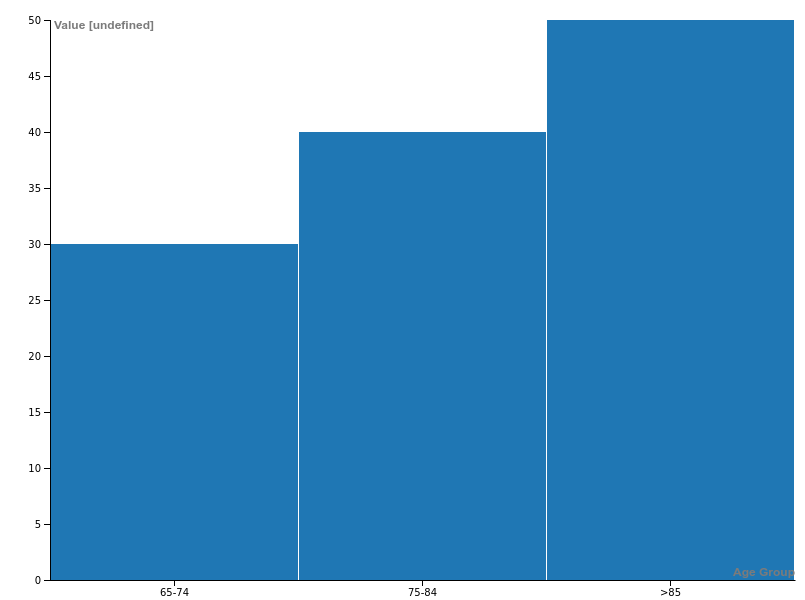
\includegraphics[width=\textwidth]{images/fall_status_who.png}
                \caption{Tỷ lệ té ngã theo nhóm tuổi}
            \end{figure}
        \end{column}
    \end{columns}
\end{frame}

\subsection{TỔNG QUAN CÁC PHƯƠNG PHÁP CÁC PHƯƠNG PHÁP  PHÁT HIỆN TÉ NGÃ} 
% --- Slide 4: Tổng quan các phương pháp ---
\begin{frame}{Tổng quan các phương pháp phát hiện té ngã}
    \begin{itemize}
        \item \textbf{Dựa trên thị giác (Vision-based)}: Sử dụng camera và thuật toán nhận diện tư thế người (MediaPipe, OpenPose).
        \item \textbf{Dựa trên cảm biến đeo (Wearable-based)}: Dùng cảm biến quán tính (IMU, MPU6050) trên thiết bị.
        \item \textbf{Kết hợp đa phương thức (Multi-modal)}: Tích hợp dữ liệu từ nhiều nguồn để tăng độ chính xác.
    \end{itemize}
\end{frame}

